\chapter{ƯỚC TÍNH TỌA ĐỘ KHUNG XƯƠNG TỪ ẢNH RGB}
\label{s:pose estimate}
Trong nội dung này, em sẽ trình bày hai phương pháp đề xuất để trích xuất đặc trưng khung xương. Đó là trích xuất đặc trưng từ thiết bị Kinect và trích xuất đặc trưng từ mạng neuron network. Phương pháp trích xuất đặc trưng khung xương từ ảnh RGB qua mạng NN dựa trên mạng mobilenet v2 được áp dụng trong đề tài vì tính khả thi, có thể ứng dụng được trong đời sống cao hơn so với phương pháp sử dụng camera Kinect.

\section{ƯỚC TÍNH DỰA TRÊN CAMERA ĐỘ SÂU KINECT}
\label{ss:kinect}
\subsection{Giới thiệu camera cảm biến độ sâu Kinect của Microsoft}
Kinect là một thiết bị đầu vào,là cảm biến chuyển động do hãng Microsoft sản xuất dành cho Xbox 360 và máy tính Windows. Dựa trên một webcam kiểu add-on ngoại vi cho Xbox 360, nó cho phép người dùng điều khiển và tương tác với Xbox 360 mà không cần phải dùng đến một bộ điều khiển tay cầm, thông qua một giao diện người dùng tự nhiên bằng cử chỉ và lệnh nói. Thiết bị được giới thiệu vào tháng 11 năm 2010 như một phụ kiện của Xbox 360. Cảm biến chiều sâu (depth sensor) được sử dụng trong Kinect được lấy từ việc trích xuất camera hồng ngoại. 

Chức năng chính của Kinect là một công cụ để người dùng tương tác với Xbox 360 bằng cử chỉ và lệnh nói. Vì lý do này, các bộ cảm biến có khả năng thu thập dữ liệu ở độ phân giải 640x480 điểm ảnh. Với các dữ liệu chiều sâu, có thể lấy được "các vector đặc trưng mang hình dáng của khung xương con người(SJMs)" của người đứng phía trước của cảm biến. Và với các SJM đó, nó có thể nhận biết được cử chỉ của người sử dụng.

\FloatBarrier
\begin{figure}[htp]
\begin{center}
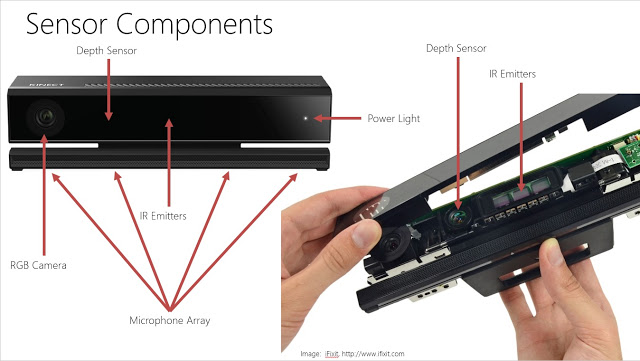
\includegraphics[scale=0.8]{chap3/c3_figs/kinect.png}
\end{center}
\caption{Camera cảm biến độ sâu Kinect \\(Nguồn : \url{https://www.ifixit.com)}}
\label{fig:kinect}
\end{figure}
\FloatBarrier

Các thông số cơ bản của cảm biến như sau:
\begin{itemize}
\item Ảnh màu : 1920x1080 @30Hz (15Hz ánh sáng yếu)
\item Ảnh độ sâu : 512x424 @30Hz
\item Tầm xa : 0.5 $\sim$ 4.5m
\item Góc nhìn (Dọc/Ngang) : 70 / 60 độ
\item Số lượng SJM (phát hiện/theo dõi) : 6 / 6 SJMs
\item Số lượng SJM-J : 25 SJM-Js
\item Hệ điều hành : Windows 8/10
\item Cổng tín hiệu : USB 3.0
\end{itemize}

Cơ chế hoạt động: Ban đầu, bộ phần phát tia hồng ngoại sẽ phát ra tia hồng ngoại trong vùng hoạt động của nó. Thông qua phản chiếu các tia hồng ngoại về camera hồng ngoại sẽ thu nhận được các tia phản xạ về. Dựa vào thời gian trễ để đo khoảng cách tới các điểm trong vùng quan sát. Kết quả thu về sẽ là hình ảnh vùng quan sát với những chiều sâu khác nhau.

\FloatBarrier
\begin{figure}[htp]
\begin{center}
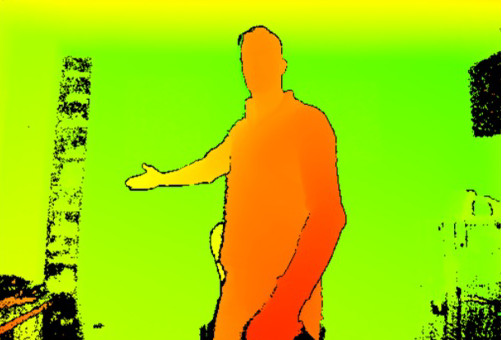
\includegraphics[scale=0.8]{chap3/c3_figs/depth.jpg}
\end{center}
\caption{Ảnh độ sâu từ Kinect \\(Nguồn : \url{https://www.zonetrigger.com/)}}
\label{fig:kinect}
\end{figure}
\FloatBarrier

\subsection{Cơ chế trích xuất SJM từ Kinect}
Ưu điểm của việc sử dụng Kinect là các thiết kế phần cứng đã tối ưu cho việc tạo ra SJM, không yêu cầu phải thực hiện lại hoặc tạo ra thuật toán mới cho phần trích xuất đặc trưng. Sơ đồ khối trích xuất SJM của Kinect v2 minh họa bằng hình \ref{fig:TrichKhungXuong}.

\FloatBarrier
\begin{figure}[htp]
\begin{center}
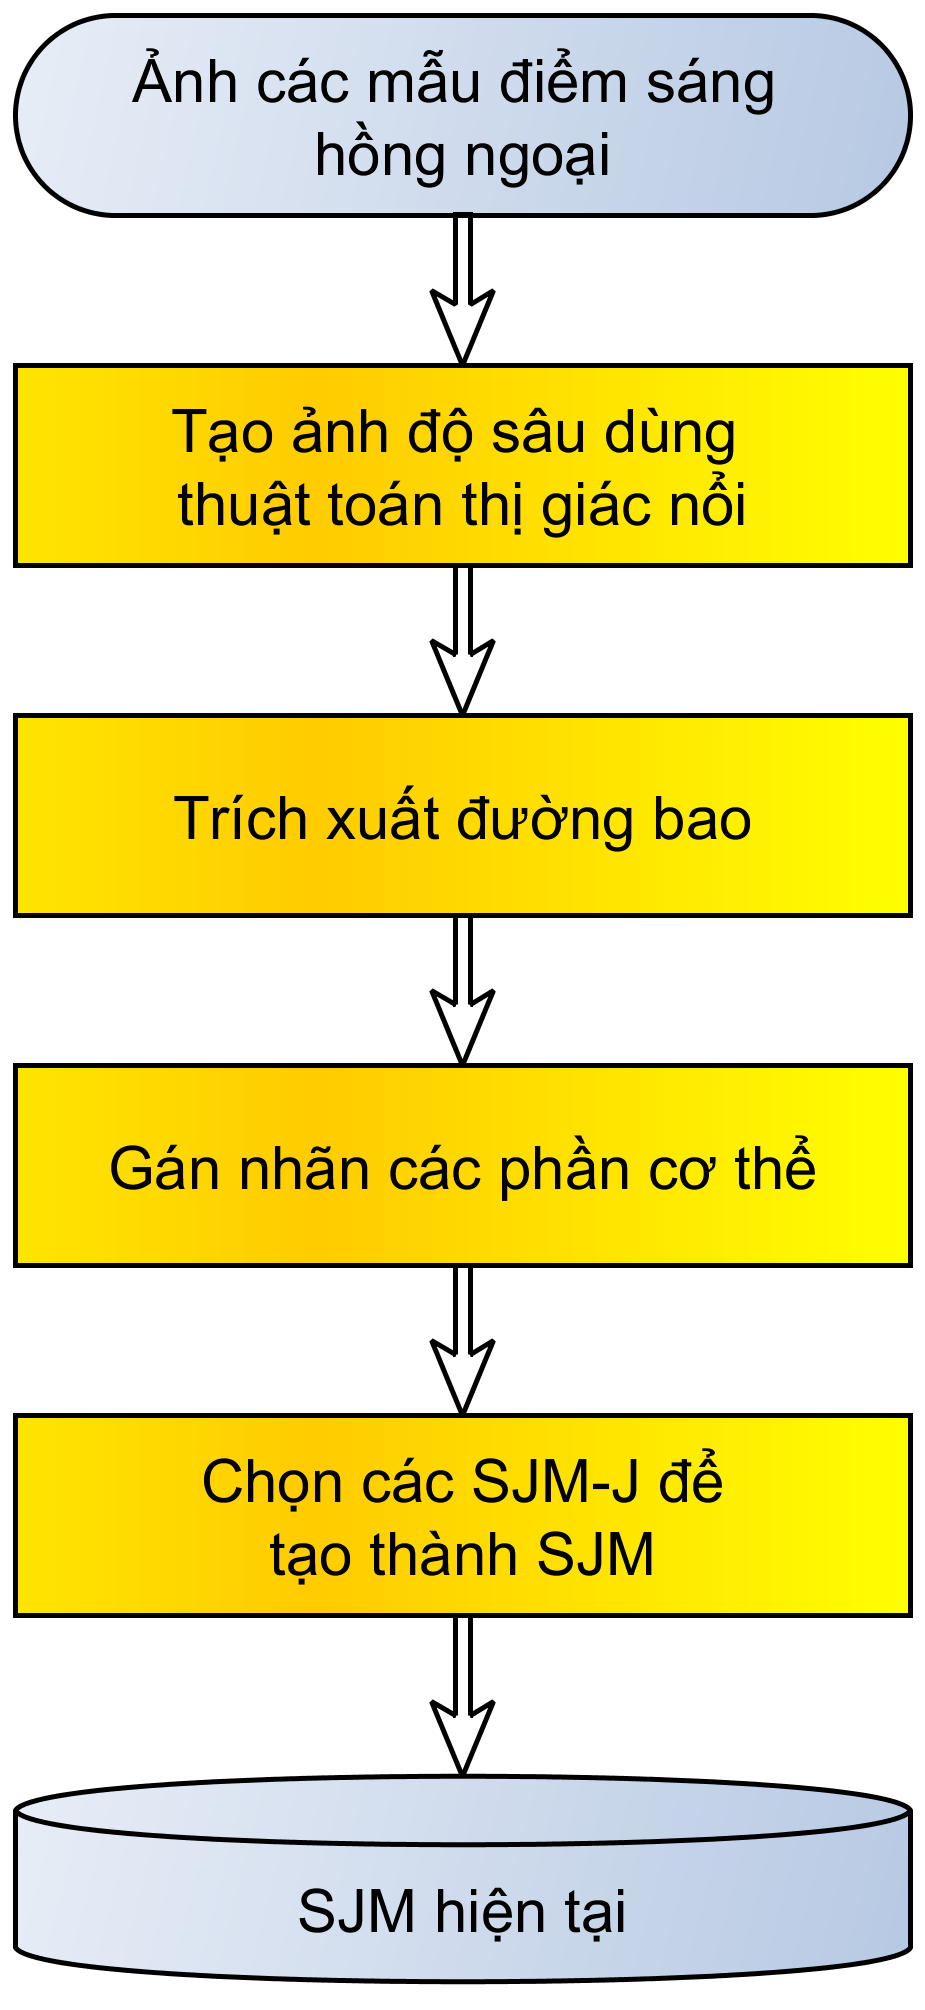
\includegraphics[scale=0.15]{chap3/c3_figs/TrichKhungXuong.png}
\end{center}
\caption{Sơ đồ khối thuật toán trích xuất SJM của thiết bị Kinect \\(Nguồn : "Nhận dạng ngôn ngữ ký hiệu cho người câm" - B.V Phúc, H.C Thịnh)}
\label{fig:TrichKhungXuong}
\end{figure}
\FloatBarrier

\underline{\textbf{Dữ liệu ngõ vào}}

Hành động di chuyển của người dùng trong không gian nhận diện được của thiết bị Kienct v2.

\underline{\textbf{Dữ liệu ngõ ra}}
\begin{itemize}
\item Ảnh màu kých thước 1920x1080 pxs.

\item Ảnh biểu diễn độ sâu 512x424 pxs.

\item SJM tương ứng với ảnh hiện tại biễu diễn tọa độ bằng meter (đo tương đối bằng ảnh độ sâu) hoặc px (tương ứng với vị trí của ảnh độ sâu).
\end{itemize}

Sau khi ước tính tọa độ khung xương bằng Kinect, ta thu được tọa độ các vị trí của 25 khớp xương trong không gian 3 chiều (hình \ref{fig:skeleton_kinect})

\FloatBarrier
\begin{figure}[htp]
\begin{center}
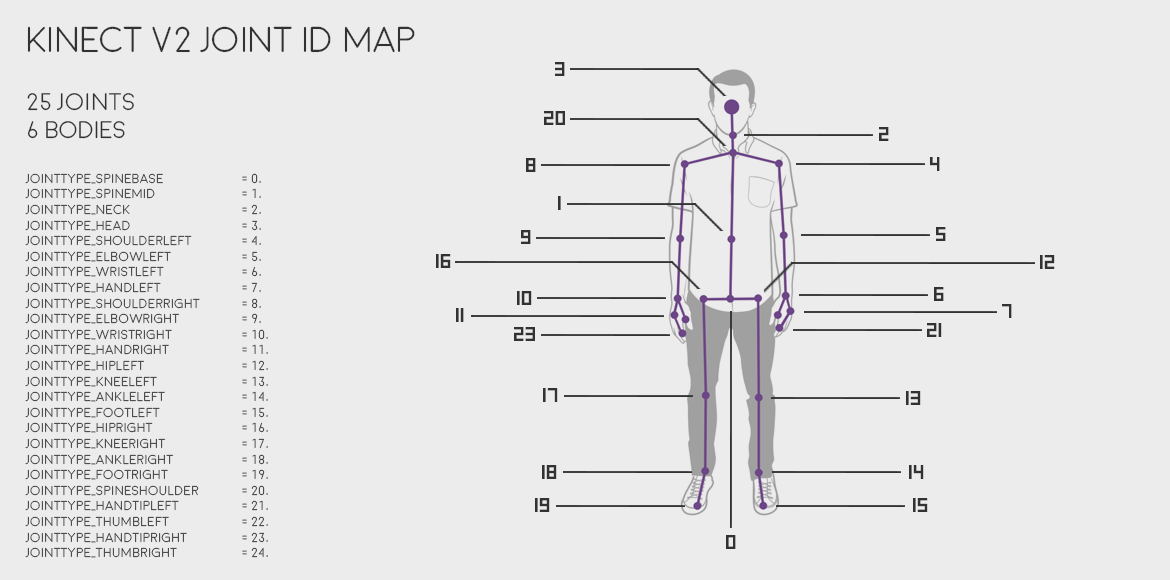
\includegraphics[scale=0.4]{chap3/c3_figs/kinectskeleton.png}
\end{center}
\caption{Khung xương được trích xuất từ Kinect \\(Nguồn : \url{https://www.zonetrigger.com/)}}
\label{fig:skeleton_kinect}
\end{figure}
\FloatBarrier

Việc ước tính tọa độ khung xương dựa trên camera Kinect mang nhiều ưu điểm như tốc độ ước tính nhanh do phần cứng đã tối ưu việc xử lý khớp xương. Kết quả ước tính trên không gian 3 chiều mang độ chính xác cao giúp cho các ứng dụng dựa trên ước tính tọa độ khung xương thực hiện tốt. Tuy nhiên luận văn áp dụng mô hình ước tính tọa độ khung xương dựa vào mạng NN giúp áp dụng vào các thiết bị camera RGB bình thường dễ dàng hơn. Phần tiếp theo luận văn xin trình bày về mạng Neural network này.

\section{ƯỚC TÍNH TỪ ẢNH 2D DỰA TRÊN MẠNG NEURAL NETWORK}
\label{ss:2Dpose}
\subsection{Tổng quan phương pháp}
\label{sss:tong_quan_2D_pose}
Phương pháp trích xuất hình dáng khung xương được áp dụng từ bài báo "Realtime Multi-Person 2D Pose Estimation using Part Affinity Fields" \cite{cao2017realtime} sử dụng phương pháp bottom-up ước tính tọa độ khung xương từ ảnh sang không gian 2D. Tuy có rất nhiều mạng pose estimate cả 2D lẫn 3D và cả dense pose(ước tính toàn bộ hình dáng cơ thể người) nhưng phương pháp ước tính 2D được chọn vì tốc độ xử lý có thể đáp ứng realtime và hoạt động trên các thiết bị cấu hình thấp. Ngoài ra phương pháp này có thể ước tính tọa độ khung xương nhiều người cùng một lúc 

Mạng sử dụng  detect tư thế 2D song song của nhiều người trong một ảnh. Phương pháp sử dụng một đại diện không có thông số "trường ái lực một phần" (PAFs) được tham khảo để học cách liên kết các bộ phần cơ thể với mỗi cá nhân trong ảnh. Mô hình mã hóa toàn bộ bối cảnh, cho phép một bước phân tích từ dưới lên trên (bước này có độ chính xác cao, realtime và thực hiện song song nhiều người). Mô hình được thiết kế để kết hợp tìm vị trí các phần và liên kết giữa chúng thông qua 2 nhánh của quá trình dự đoán chuỗi giống nhau. Phương pháp này đã đạt giải nhất tại cuộc thi COCO 2016 keypoints challenge và vượt trội hơn so với kết quả trước đó trong MPII Multi-Person benchmark về performance và sự hiệu quả.

%\subsection{Kiến trúc mạng}
%\label{sss:method}

\FloatBarrier
\begin{figure}[htp]
\begin{center}
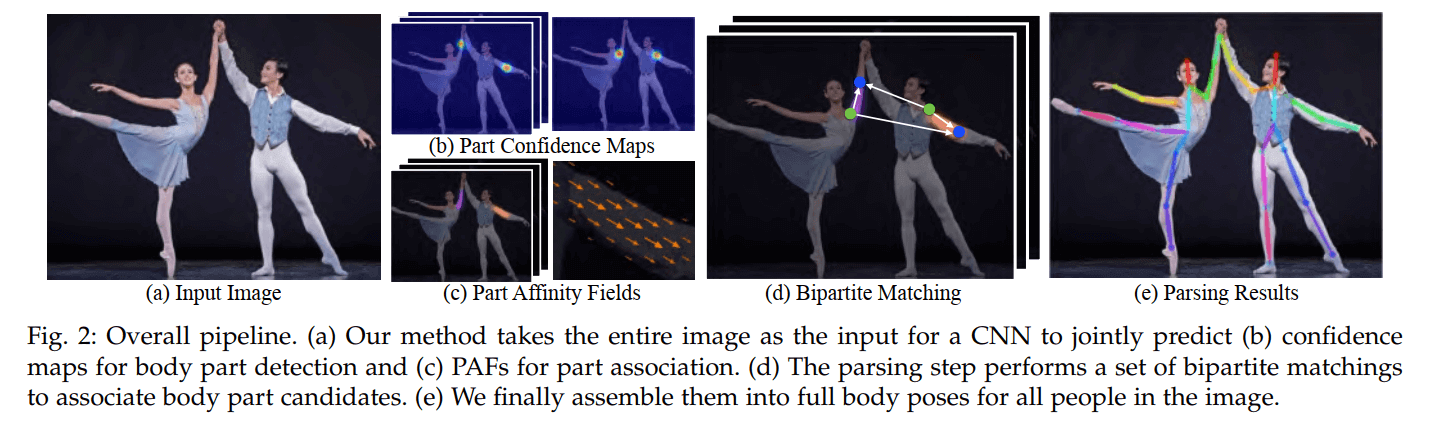
\includegraphics[scale=0.3]{chap3/c3_figs/pipeline.png}
\end{center}
\caption{Tổng thể kiến trúc}
\label{fig:pipeline}
\end{figure}
\FloatBarrier

Hình \ref{fig:pipeline} mình họa toàn bộ nội dung phương pháp. Hệ thống lấy đầu vào, một ảnh màu có kích thước $w*h$ (hình \ref{fig:pipeline}a) và tạo ra ngõ ra, tọa độ của những keyponts cho mỗi cá nhân trong ảnh (hình \ref{fig:pipeline}e). Đầu tiên, một mạng CNN đồng thời dự đoán một loạt những confidence maps (cfm) S của những vị trí bộ phận cơ thể (hình \ref{fig:pipeline}b) và một loạt những miền vector 2D (vf) L của part affinities, cái mà mã hóa độ liên kết giữa các phần cơ thể (hình \ref{fig:pipeline}c). Tập hợp  có J cfm, một map cho mỗi bộ phận, trong đó . Tập hợp  có C vf, một cho mỗi chi, trong đó , mỗi vị trí ảnh trong Lc mã hóa một vector 2D (được show trong hình 1). Cuối cùng, cfm và affinity fields được phân tích bởi suy luận tham lam (hình \ref{fig:pipeline}d) để tạo ra các keypoints 2D cho tất cả người trong ảnh.

Phương pháp này đưa toàn bộ ảnh đầu vào qua một mạng CNN 2 nhánh để đồng thời dự đoán những confidence map cho sự detect phần cơ thể, thể hiện trong hình \ref{fig:pipeline}b, và part affinity fields cho sự liên kết các phần, thể hiện trong hình \ref{fig:pipeline}c. Bước phân tích thể hiện một loạt những liên kết giữa hai điểm (liên kết lưỡng cực) để liên kết những phần cơ thể (\ref{fig:pipeline}d). Cuối cùng, chúng được lắp ráp chúng lại với nhau tạo thành những tư thế cơ thể hoàn chỉnh cho tất cả những người trong ảnh (\ref{fig:pipeline}e).

\begin{itemize} % chấm đầu dòng
\item Đầu tiên, hình ảnh được truyền qua mạng cơ sở để trích xuất các bản đồ đặc trưng. Trong bài báo, tác giả sử dụng 10 lớp đầu tiên của mô hình VGG-19. Tuy nhiên model được luận văn áp dụng sử dụng 10 lớp đầu tiên của mô hình mobilenet\_v2 model này gọn nhẹ hơn so với VGG-19 nên có thể đáp ứng realtime đối với các máy tính cấu hình thấp.
\end{itemize}


\begin{itemize} % chấm đầu dòng
\item Sau đó, các bản đồ tính năng được xử lý với nhiều giai đoạn CNN để tạo: một bộ Bản đồ tin cậy một phần và một bộ các trường có mối quan hệ một phần (PAF)
	\begin{itemize}
	\item \textbf{Confidence Maps} : một bộ bản đồ độ tin cậy 2D S cho các vị trí phần cơ thể. Mỗi vị trí chung có một bản đồ.
	\item \textbf{Part Affinity Fields} : một tập hợp các trường vectơ 2D L mã hóa mức độ liên kết giữa các phần.
	\end{itemize}
\end{itemize}


\begin{itemize} % chấm đầu dòng
\item Cuối cùng, \textbf{Confidence Maps} và \textbf{Part Affinity Fields} được xử lý bằng thuật toán tham lam để có được tư thế cho mỗi người trong ảnh.
\end{itemize}

\subsection{Giải thích các phần}
%\renewcommand{\labelitemi}{$\square$}
%\renewcommand\labelitemii{$\nabla$}
%\renewcommand\labelitemiii{$\square$}
\begin{itemize}
  \item[$\square$] \textbf{Confidence Maps (CFMs)} là một đại diện 2D cho niềm tin rằng một bộ phận cơ thể cụ thể có thể được đặt trong bất kỳ pixel nào. Với J là số lượng vị trí bộ phận cơ thể (khớp). Sau đó, \textbf{Confidence Maps} $S = (S_1, S_2, .., S_J)$ với $S_j \in R^{w \times h},j \in (1 \ldots J)$
  Tóm lại, mỗi bản đồ tương ứng với một khớp và có cùng kích thước với hình ảnh đầu vào .

  \item[$\square$] \textbf{Part Affinity Fields(PAF)}
  Trường quan hệ một phần \textbf{(PAF)} là một tập hợp các trường dòng mã hóa các mối quan hệ cặp đôi không cấu trúc giữa các bộ phận cơ thể.

Mỗi cặp bộ phận cơ thể có một \textbf{PAF} , tức là cổ, mũi, khuỷu tay, v.v.

Cho $C$ là số lượng các cặp phần trên cơ thể. Sau đó \textbf{PAFs} là các thiết lập \textbf{$L = (L_1, L_2, ..., L_c)$} với \textbf{$L_c \in R^{w \times h \times 2},c \in (1 \ldots C)$}

Nếu một pixel nằm trên một chi (phần cơ thể), giá trị trong $L_c$ tại pixel đó là một vectơ đơn vị 2D từ khớp bắt đầu đến khớp cuối.
\item[$\square$] \textbf{CNN nhiều giai đoạn}

\FloatBarrier
\begin{figure}[htp]
\begin{center}
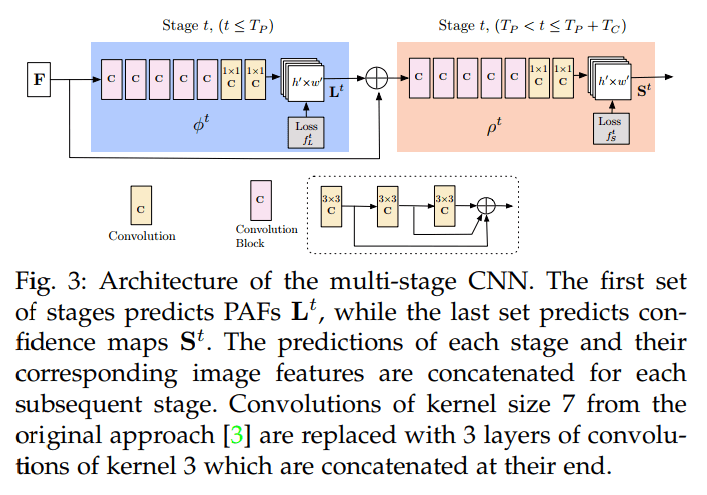
\includegraphics[scale=0.65]{chap3/c3_figs/CNN_m.png}
\end{center}
\caption{Kiến trúc của CNN nhiều giai đoạn từ phiên bản tạp chí của OpenPose}
\label{fig:CNN_multi_stage}
\end{figure}
\FloatBarrier

\textbf{CNN nhiều giai đoạn gồm các bước như sau:}
\begin{itemize}
\item Tính toán các \textbf{part affinity fields (PAFs)}, $ L^{1}$ từ feature maps của mạng cơ sở $F$. Cho $\phi^1$ là mạng CNN mạng CNN tại bước 1. 
$$L^1 = \phi^1(F) $$

\item Giai đoạn $t$ đến giai đoạn $T_P$: Tinh chỉnh dự đoán của \textbf{PAF} từ giai đoạn trước bằng cách sử dụng bản đồ tính năng $F$ và các \textbf{PAF} trước đó $(L^{t-1})$.Với $\phi^t$ là CNN ở giai đoạn t.
$$L^t = \phi^t(F, L^{t-1}), \forall 2 \leq t \leq T_P$$
\item Sau khi $T_P$ lặp đi lặp lại, quá trình được lặp lại việc phát hiện \textbf{confidence maps} , bắt đầu trong dự đoán PAF cập nhật mới nhất . $\rho^t$ là CNN ở giai đoạn $t$. Quá trình được lặp lại cho $T_C$.
$$S^{T_P} = \rho^t(F, L^{T_P}), \forall t = T_P$$
$$S^t = \rho^t(F, L^{T_P}, S^{t-1}), \forall T_P \leq t \leq T_P + T_C$$

\item Ma trận $S$ và $L$ cuối cùng là \textbf{Confidence Maps} và \textbf{part affinity fields (PAFs)} sẽ được xử lý thêm bằng thuật toán tham lam.

\end{itemize}
\end{itemize}
\textbf{Chú thích:}
CNN nhiều giai đoạn này là từ phiên bản tạp chí 2018. Trong phiên bản CVPR 2017 gốc, họ đã tinh chỉnh cả bản đồ độ tin cậy và các trường mối quan hệ một phần (PAF) ở mỗi giai đoạn. Do đó, họ đòi hỏi nhiều tính toán và thời gian hơn ở mỗi giai đoạn. Trong cách tiếp cận mới, tác giả nhận thấy rằng cách tiếp cận mới làm tăng cả tốc độ và độ chính xác tương ứng 200\% và 7\%.

\subsection{Kiến trúc mạng}
\label{sss:structure}
\subsubsection{Phát hiện và liên kết đồng thời}

Kiến trúc của mạng, được show trong hình \ref{fig:structure}, dự đoán đồng thời những cfm và affinity fields \textbf{(af)} cái mà mã hóa liên kết giữa các phần. Mạng được tách thành 2 nhánh: Nhánh trên, màu hường da, dự đoán những \textbf{cfm}, và nhánh dưới, màu xanh, dự đoán những \textbf{af}. Mỗi nhánh là một kiến trúc dự đoán lặp lại, theo như \ref{wei2016convolutional}, nó tinh chỉnh những dự đoán qua các giai đoạn liên tiếp $t \in {{1 \ldots T}}$,  với giám sát trung gian ở từng giai đoạn.

\FloatBarrier
\begin{figure}[htp]
\begin{center}
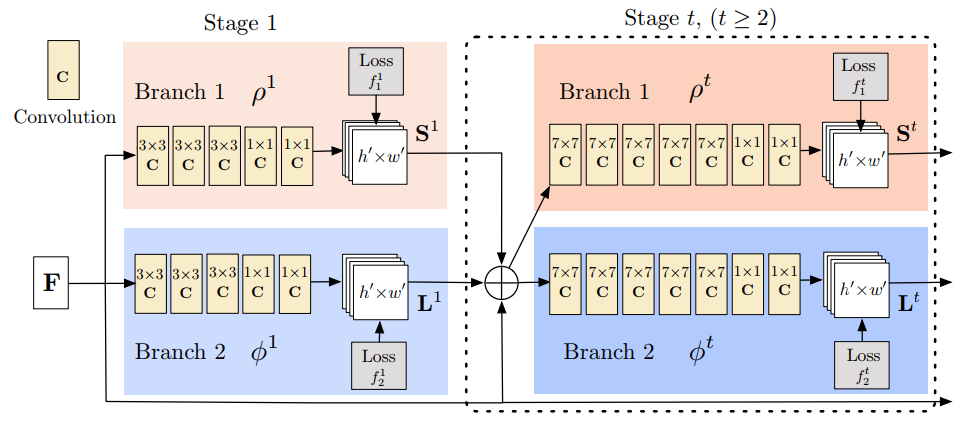
\includegraphics[scale=0.45]{chap3/c3_figs/structure.png}
\end{center}
\caption{Kiến trúc của mạng CNN nhiều bước 2 nhánh. Mỗi bước trong nhánh đầu tiên dự đoán những $CFM S^{t}$, và mỗi bước trong nhánh thứ 2 dự đoán $PAFs L^{t}$. Sau mỗi bước, những dự đoán từ 2 nhánh, cùng với những đặc trưng ảnh, được nối lại cho bước tiếp theo.}
\label{fig:structure}
\end{figure}
\FloatBarrier

\subsection{Phân tích nhiều người sử dụng PAFs}
\label{ss:Multi-Person Parsing using PAFs}

Trong phần này, sẽ nói về tổng quan về thuật toán tham lam được sử dụng để phân tích tư thế của nhiều người từ PAFs và CFMs.

Quá trình phân tích được tóm tắt thành 3 bước sau:
\begin{itemize}
\item Bước 1: Tìm tất cả những vị trí khớp sử dụng confidence maps.
\item Bước 2: Tìm những khớp cùng nhau tạo các chi (bộ phận cơ thể) sử dụng PAFs và những khớp trong bước 1.
\item Bước 3: Kết nối các chi thuộc cùng một người và tạo danh sách những tư thế cơ thể.
\end{itemize}

\subsubsection{Bước 1 - Tìm tất cả những vị trí khớp sử dụng confidence maps.}
\begin{itemize}
\item \textbf{Đầu vào:}
	\begin{itemize}
	\item Confidence maps, $S = (S_1, S_2, .., S_J)$ trong đó $S_j \in R^{w \times h},j \in (1 \ldots J)$.
	\item Up-sampling scale: Sự khác biệt giữa dài/rộng giữa ảnh đầu vào và confidence maps.
	\end{itemize}
\item \textbf{Đầu ra: }
	\begin{itemize}
	\item Danh sách khớp(joints$\_$list): một danh sách những vị trí khớp của kích thước J, mỗi phần tử là một danh sách các đỉnh (x, y, xác suất).
	\item Ví dụ, kích thước của joints$\_$list là 18 cho 18 vị trí khớp (mũi, cổ,...) và những phần tử trong joints$\_$list là những danh sách có độ dài khác nhau. Những phần tử này lưu trữ thông tin đỉnh (vị trí x, y và điểm xác suất) cho mỗi vị trí khớp.
	\end{itemize}
\item \textbf{Xử lý: Cho mỗi khớp từ 1 dến J:}
	\begin{itemize}
	\item Lấy heatmap 2D tương ứng cho khớp trong confidence maps.
	\item Tìm những đỉnh bằng cách lấy ngưỡng heatmap 2D.
	\item Đối với mỗi đỉnh:
		\begin{itemize}
		\item Lấy một đốm xung quanh đỉnh trong heap.
		\item Phóng to đốm sử dụng up-sampling scale.
		\item Lấy vị trí đỉnh lớn nhất trong đốm được phóng to.
		\item Thêm thông tin đỉnh vào danh sách các đỉnh của khớp.
		\end{itemize}
	\end{itemize}
\end{itemize}

\subsubsection{Bước 2 - Tìm những khớp cùng nhau tạo các chi (bộ phận cơ thể) sử dụng PAFs và những khớp trong bước 1.}
\begin{itemize}
\item \textbf{Đầu vào:}
	\begin{itemize}
	\item joints-list ngõ ra của bước 1.
	\item \textbf{PAFs}: \textbf{$L = (L_1, L_2, ..., L_c)$} trong đó \textbf{$L_c \in R^{w \times h \times 2},c \in (1 \ldots C)$}
	\item  Up-sampling scale: sự khác nhau giữa dài rộng của ảnh đầu vào và PAFs maps.
	\item Số lượng những điểm trung gian: số lượng những điểm trung gian giữa một khớp nguồn và những khớp đích để có được giá trị PAFs.
	\end{itemize}
%\end{itemize}
\item \textbf{Đầu ra: }
	\begin{itemize}
	\item Những chi được kết nối (connected-limbs): một danh sách những chi được kết nối có kích thước C. Trong đó, mỗi phần tử là một danh sách tất cả các chi của loại đó.
	\item Mỗi thông tin chi chứa: id của chi nguồn, id của chi đích và điểm số thể hiện độ tốt của kết nối.
	\end{itemize}
\item \textbf{Xử lý: }
	\begin{itemize}
	\item  Phóng to PAFs đến kích thước của ngõ vào sử dụng up-sampling scale.
	\item Đối với mỗi loại chi, ví dụ cổ tay-khuỷu tay trái:
		\begin{itemize}
		\item Lấy tất cả những đỉnh khớp nguồn và những đỉnh khớp đích, ví dụ: tất cả những đỉnh cổ tay trái và tất cả những đỉnh khuỷu tay trái.
		\item Nếu kích thước của những đỉnh nguồn hoặc đỉnh đích bằng 0, thì bỏ qua chi đó.
		\item Tạo một danh sách để lưu trữ tất cả những candidates kết nối chi.
		\item Đối với mỗi đỉnh nguồn và mỗi đỉnh đích:
			\begin{itemize}
			\item Lấy vector trực tiếp bằng cách trừ những vị trí nguồn và vị trí đích.
			\item Chuẩn hóa vector trực tiếp thành vector đơn vị.
			\item  Lấy giá trị PAFs tại mỗi điểm trung gian giữa những đỉnh nguồn và đỉnh đích.
			\item Tính điểm số của kết nối chi hiện tại bằng cách lấy trung bình những giá trị PAFs.
			\item Thêm điểm số để xác định khoảng cách chi phù hợp:  
			
			\textbf{min(0.5 * paf\_height / limb\_dist - 1, 0)}.
			\item Thêm những kết nối chi hiện tại vào những candidates kết nối chi:
			
			+ Sắp xếp những candidates kết nối chi.
			
			+ Đối với mỗi candidate kết nối chi: Thêm sự kết nối vào danh sách cuối cùng nếu nguồn và đích không được chọn cho bất kỳ sự kết nối nào.
			\end{itemize}
		\end{itemize}
	\end{itemize}
\end{itemize}

\subsubsection{Bước 3 - Kết nối các chi thuộc cùng một người và tạo danh sách những tư thế cơ thể.}
\begin{itemize}
\item \textbf{Đầu vào:}
	\begin{itemize}
	\item Danh sách khớp (\textbf{joint$\_$list}) từ bước 1.
	\item Những chi được kết nối (connected$\_$limbs) từ bước 2
	\end{itemize}
\item \textbf{Đầu ra:} Những tư thế: một danh sách những tư thế người cho mỗi các nhân trong ảnh. Mỗi phần từ chứa những vị trí khớp cho người đó.
\item \textbf{Xử lý:}
	\begin{itemize}
	\item Đối với mỗi loại chi và đối với mỗi kết nối giữa các chi (connected\_limbs) của loại đó:
		\begin{itemize}
		\item Tìm những cá nhân liên kết với khớp của kết nối hiện tại.
		\item Nếu không có người nào: Tạo một người mới với kết nối hiện tại.
		\item Nếu có một người: Thêm kết nối hiện tại vào người đó.
		\item Nếu có 2 người: Xác nhập 2 người này thành một người.
		\end{itemize}
	\item Loại bỏ những người có quá ít khớp.
	\end{itemize}
\end{itemize}

\subsection{Kết quả}
Ảnh RGB đầu vào chứa nhiều người sau khi xử lý qua mạng ta nhận được tọa độ 18 khớp xương của từng người được vẽ ra trên ảnh đầu ra. Kết quả ước lượng có thể đáp ứng được xử lý thời gian thực (realtime) trên máy tính cấu hình thấp với FPS đạt được khoảng 2.5 -> 4(FPS). Tốc độ nhận dạng tùy thuộc vào số người trong khung hình, tốc độ xử lý sẽ càng nhanh khi số lượng người trong khung hình càng ít và ngược lại.

\FloatBarrier
\begin{figure}[htp]
\begin{center}
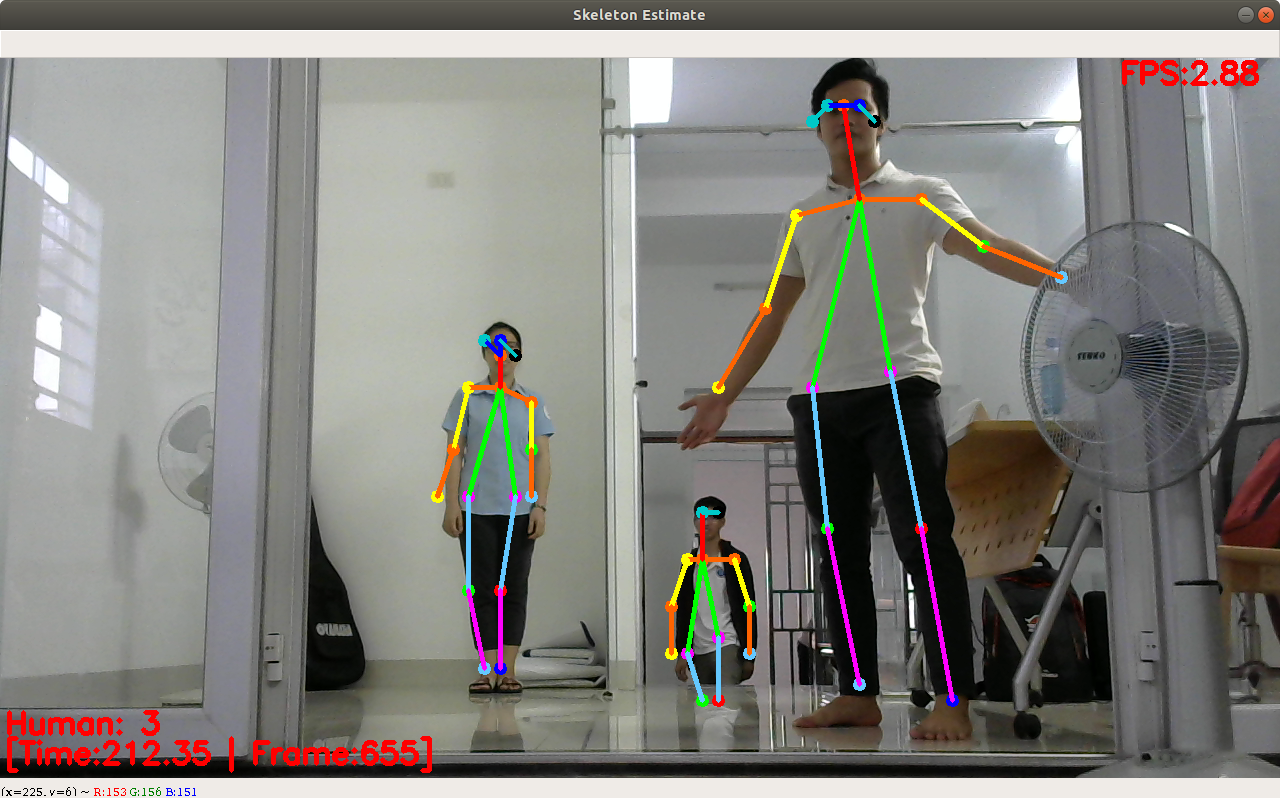
\includegraphics[scale=0.37]{chap3/c3_figs/skeleton_out.png}
\end{center}
\caption{Kết quả ước tính tọa độ khung xương từ mạng NN}
\label{fig:kq_skeleton}
\end{figure}
\FloatBarrier

\section{Kết luận}
Ước lượng khung xương hay ước tính tư thế con người là một hướng nghiên cứu quan trọng và đầy thách thức của thị giác máy tính. Phương pháp này được khá nhiều nghiên cứu áp dụng để giải quyết nhiều bài toán khó như nhận dạng dáng đi, tư thế con người, nhận dạng hành động hay giúp robot học theo chuyển động của con người...Chương tiếp theo, luận văn sẽ trình bày về ứng dụng của ước lượng tọa độ khung xương trong nhận dạng ngôn ngữ ký hiệu, là phần nghiên cứu chính của luận văn.